\chapter{Evaluation}
\label{cpt:evaluation}
In this section, the results for different analytical evaluations are presented.
At first, an overview about the utilized \abr{DDS} subset is described and the necessity of each feature is justified.
This is followed by an evaluation of the system, which is subdevided into an evaluation of the system's structure, composed of its components and network topology, as well as an implementation evaluation.
Within the implementation evaluation, all characteristics that correspond with the manner of how the software is implemented, are considered.

\section{DDS Subset Identification}

For reducing system approving costs, it is important to limit the amount of utilized features and lines of code.
Therefore, I identified a subset of \abr{DDS} features from OpenSplice DDS that is sufficient for building a redundant system, as done in~\autoref{cpt:Implementation}.
An overview about this subset is given and justified in the following.
This overview only contains the methods and functionalities that are directly used by the application, the middleware, however, might utilize other functionalities to implement the features mentioned in this section.

\paragraph{Domain Module}
A \abr{DDS} applications main building blocks comprise a \texttt{Domain}, one or multiple \texttt{DomainParticipants}, as well as a \texttt{DomainParticipantFactory} for creating new \texttt{DomainParticipants}~\cite{omgDDSspec}.
Next to these classes, the domain module contains various functionalities, from which only the following subset is used within the exemplary implementation.

\begin{itemize}
\item \textit{DDS\_Entity\_get\_instance\_handle} Is used for aquiring an instance handle to mark it as processed in the leader's commit phase.
\item \textit{DDS\_DomainParticipant\_create\_(publisher|subscriber|topic)} Is used for creating \abr{DDS} publishers, subscribers or topics.
\item \textit{DDS\_DomainParticipant\_delete\_(publisher|subscriber|topic)} Is used for deleting \abr{DDS} publishers, subscribers or topics.
\item \textit{DDS\_DomainParticipantFactory\_get\_instance} Used for aquiring the \texttt{DomainParticipantFactory} singleton.
\item \textit{DDS\_DomainParticipantFactory\_(create|delete)\_participant} Used for creating a new participant in the \abr{DDS} domain.
\end{itemize}

Even though \textit{DDS\_DomainParticipant\_get\_default\_(publisher|subscriber|topic)\_qos} is used in the implementation, it is not mandatory because one could set the default \abr{QOS} settings directly on the corresponding entity.

\paragraph{Topic-Definition Module}
The topic definition module contains everything related to topics.
The exemplary implementation utilizes \texttt{Topics}, for describing data in the application, and \texttt{TypeSupport} which describes a data type that is bound to a \texttt{Topic}.
Next to these two classes, the following methods are used:

\begin{itemize}
\item \textit{DDS\_TypeSupport\_\_alloc} Used for creating a new \texttt{TypeSupport}.
\item \textit{DDS\_TypeSupport\_get\_type\_name} Used for getting a data type's default name, which is required to register it later on.
\item \textit{DDS\_TypeSupport\_register\_type} Used for registering a new data type name on a \texttt{DomainParticipant}.
\end{itemize}


\paragraph{Publication Module}
\texttt{Publishers}, as well as \texttt{DataWriters}, which are used for data distribution, are located within the publication module.
Besides these two classes, the following functionality is required for the exemplary implementation:

\begin{itemize}
\item \textit{DDS\_Publisher\_(create|delete)\_datawriter} Used for creating, respectively deleting, \texttt{DataWriter} objects.
\item \textit{DDS\_DataWriter\_write} Used for writing new data to an instance on a \abr{DDS} topic.
\item \textit{DDS\_DataWriter\_dispose} Used for marking processed inputs for deletion so that they are not processed twice.
\end{itemize}

\textit{DDS\_Publisher\_copy\_from\_topic\_qos} and \textit{DDS\_Publisher\_get\_default\_datawriter\_qos} are not necessarily required due to the same reasons stated above.

\paragraph{Subscription Module}
The subscription module resembles the publication module, but for reading and receiving data.
However, besides \texttt{Subscribers} and \texttt{DataReaders}, it also contains \texttt{DataSample} ,\texttt{SampleInfo}, \texttt{ReadCondition}, and \texttt{QueryCondition}, which are utilized in the exemplary implementation.
\texttt{Subscribers} and \texttt{DataReaders} are required for receiving data, which is represented by a \texttt{DataSample}.
The \texttt{SampleInfo} data structure contains additional information for each \texttt{DataSample}, such as its instance handle or state, which makes it mandatory for the implementation as well.
\texttt{ReadConditions} are used in combination with \texttt{WaitSets}, so that the application can react to certain middleware states.
\texttt{QueryConditions} are extensions for \texttt{ReadConditions} that allow to filter the data samples that are covered by a \texttt{ReadCondition}.
All filter operations could be implemented directly in the application code, whereby complexity could potential be reduced.
However, \texttt{QueryConditions} are used in the exemplary implementation because of their direct integration into other \abr{DDS} features, such as \texttt{WaitSets}.

Further, the following functionalities from the subscription module were used:

\begin{itemize}
\item \textit{DDS\_Subscriber\_(create|delete)\_datareader} Used for creating, respectively deleting, \texttt{DataReaders}.
\item \textit{DDS\_DataReader\_(create|delete)\_readcondition} Used for creating, respectively deleting, \texttt{ReadConditions}.
\item \textit{DDS\_DataReader\_create\_querycondition} Used for creating \texttt{QueryConditions}.
\item \textit{DDS\_DataReader\_take\_w\_condition} Used for reading and removing data from a \texttt{DataReader}, filtered by a \texttt{ReadCondition}.
\item \textit{DDS\_DataReader\_return\_loan} Required for indicating the middleware that the application finished accessing a sequence of data. This allows the middleware to work with the data again.
\end{itemize}

\paragraph{Infrastructure Module}
The classes that are used from the infrastructure module include \texttt{QosPolicy} and \texttt{WaitSet}.
The \texttt{QosPolicy} class implements \abr{DDS}'s \abr{QOS} functionalities and is therefore mandatory for the system's correctness.
\texttt{WaitSets} are applied for ensuring the application's compliance with its time restrictions, because they allow the assignment of timeouts.
In addition to that, the following functionalities from the infrastructure module are applied:

\begin{itemize}
\item \textit{DDS\_WaitSet\_\_alloc} Used for creating new \texttt{WaitSets}.
\item \textit{DDS\_WaitSet\_attach\_condition} Used to attach a condition to the corresponding \texttt{WaitSet}.
\item \textit{DDS\_WaitSet\_detach\_condition} Used to detach a condition from the corresponding \texttt{WaitSet}.
\item \textit{DDS\_WaitSet\_wait} Stops the according thread until at least one of the attached conditions evaluates to true.
\end{itemize}

Further, the following \abr{QOS} are applied in the application:
\todo{Add after deciding}


\section{System Evaluation}

\todo{Compare with Song et al}

\subsection{System Structure}
\begin{figure}[!hb]
	\centering
	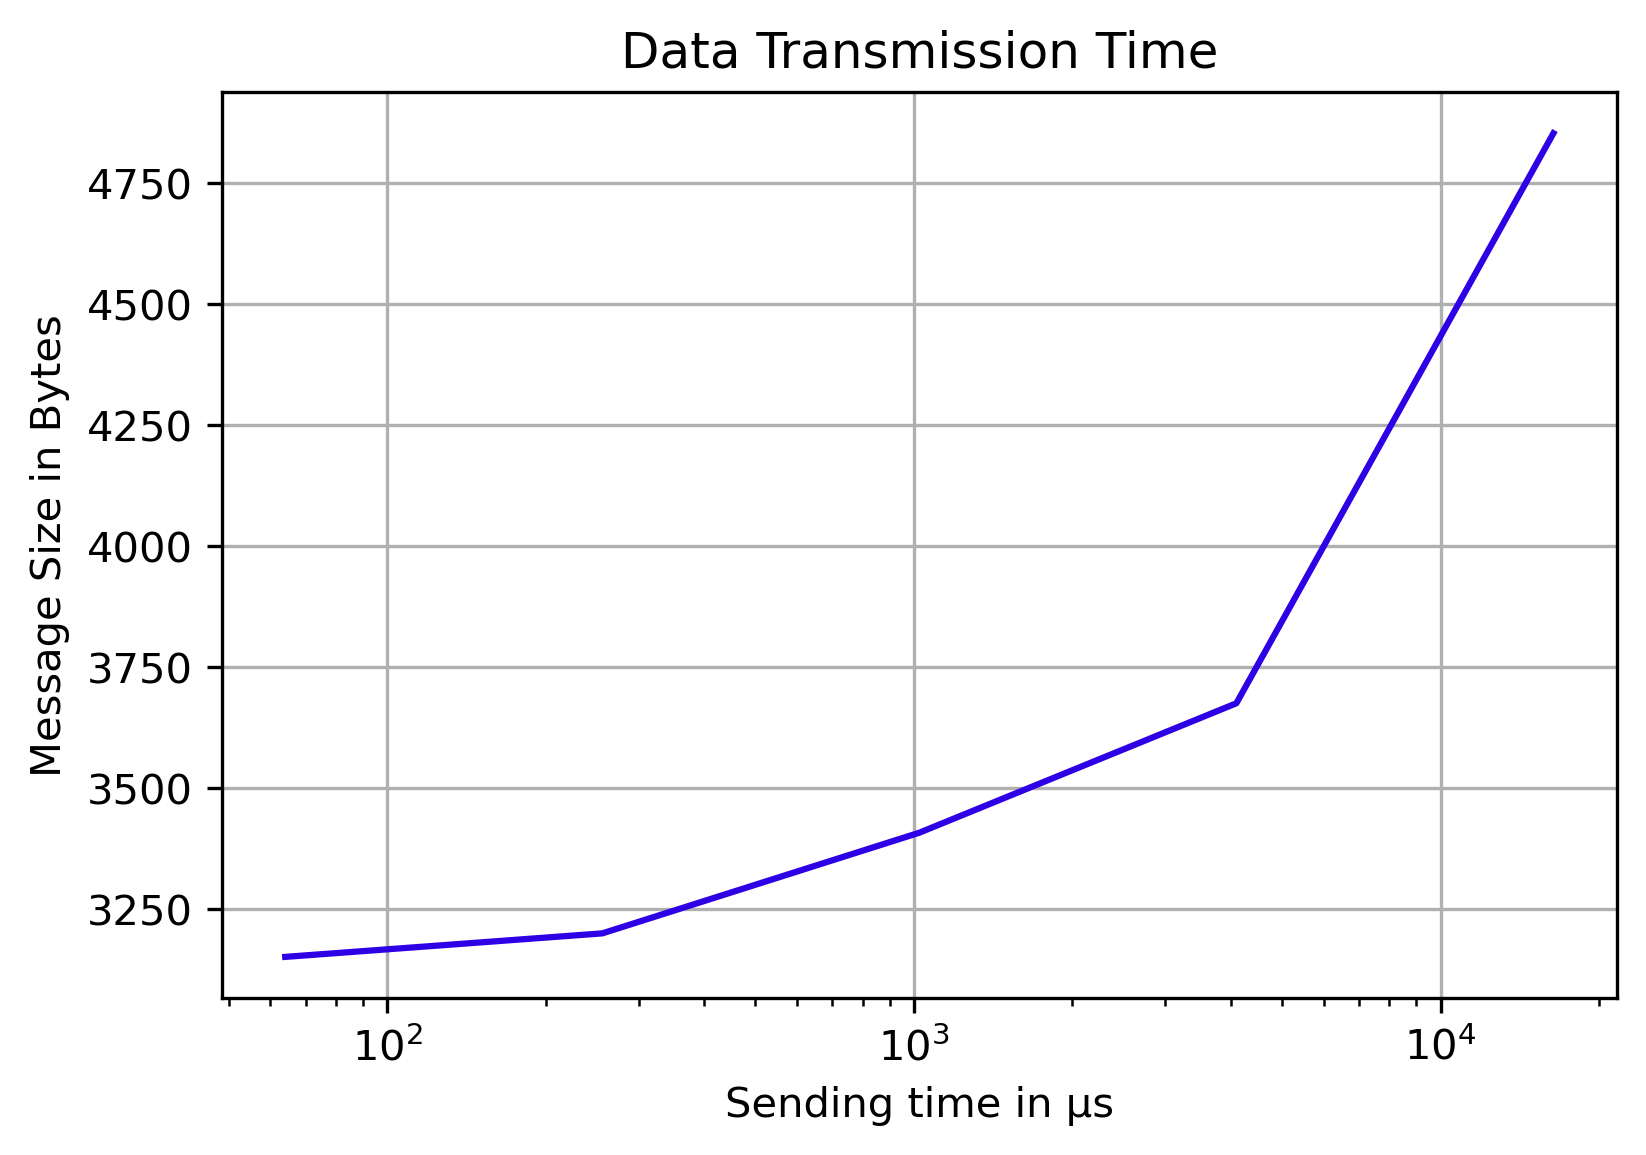
\includegraphics[width=0.75\linewidth]{images/plots/sendingTimes}
	\caption{Time that is required to transmit messages with different payload sizes via a \abr{DDS} topic. The times were determined by calculating the mean sending time out of 200 messages.}
	\label{fig:PlotSendingTimes}
\end{figure}

\paragraph{Data Transmission Time}
A end-to-end probing approach has been choosen over a \abr{IP} \abr{TTL} technique because the applied network has the same diameter for each node.
When a component publishes data to a \abr{DDS} topic, the middleware ensures that the data is transmitted to all registered subscribers.
In the system that is deployed for this thesis, data is trasmitted via \textit{Ethernet}.
The replicas are interconnected via a network switch that allows up to 2000 Mbit per seconds for each port.
In order to verify the applied topology, hardware and middleware, I measured the time that is required to send a message with a varying payload size between two replicas in the system.
For bypassing clock skews in the system, I used a request/response approach, where one replica publishes a message with a certain payload size and waits until a receiving replica confirms the message's receipt.
The receiving replica constantly checks for new messages on the system and, as soon as it receives some, publishes a confirmation messages on another topic.
Any time that is required to send the confirmation message is negligable because it only consists of a 8-bit identification number, that assigns it to a payload carrying message.
The results, which are shown in~\cite{fig:PlotSendingTimes}, were determined by measuring the time that elapsed between sending a message and receiving the corresponding confirmation.
This process was repeated 200 times for each payload size and a mean was calculated.
What emerged is, that the transmission time is directly dependent on the published message's size.
\todo{Ins verhaeltnis zur maximalen Nachrichtengroesse in meinem System setzen}

\subsection{Implementation}
\todo{Redo measurements}
\begin{figure}[!hb]
	\centering
	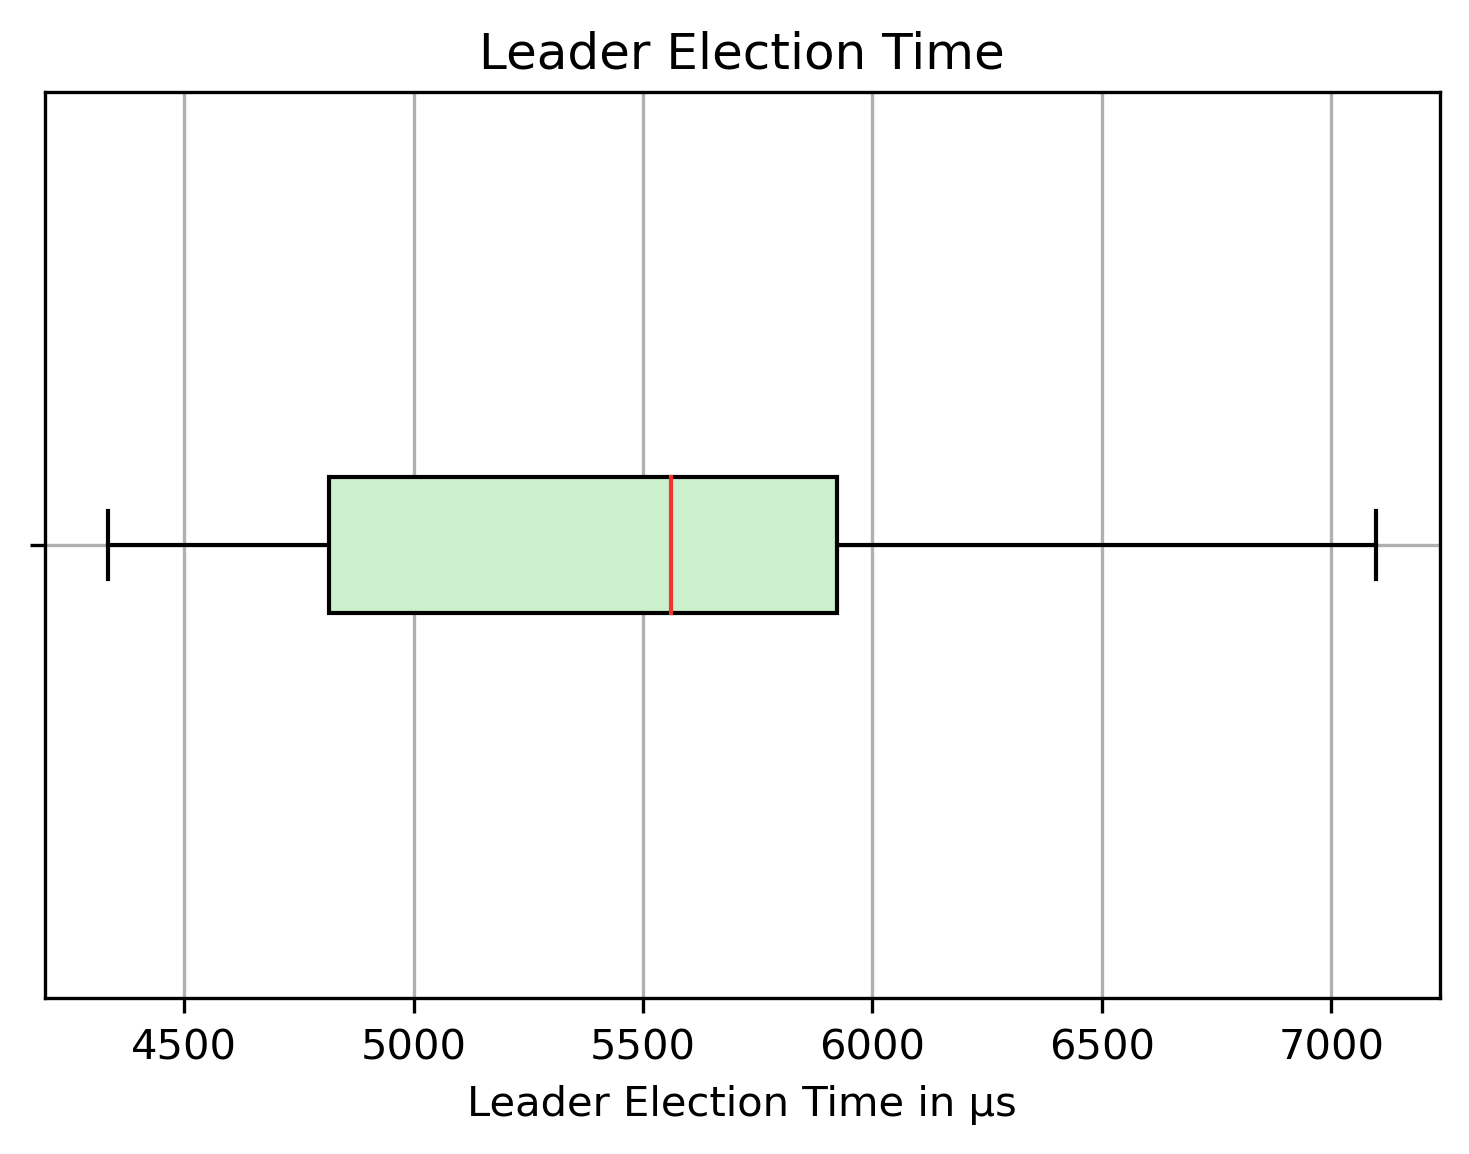
\includegraphics[width=0.75\linewidth]{images/plots/timeWithoutLeader}
	\caption{Time that the system is without a leader in each term for 20 terms. The average of 5472µs is marked by the red line.}
	\label{fig:PlotTimeWithoutLeader}
\end{figure}

\todo{Measure system utilization CPU}

\paragraph{Leader Election Time}
When the system's leader crashes, the current \texttt{Raft} term ends and a new leader gets elected.
The leader election process consists of requesting and collecting votes from all replicas in the system.
In order to make a statement about how long the system is without a leader in this case, I measured the time that elapses from when the system recognizes a missing leader until a new has send its first heartbeat message.
The results, which are depicted in~\autoref{fig:PlotTimeWithoutLeader}, show that the leader election process takes around 5500µs.
The worst election time lied aroung 7000µs.
However, since the system utilizes a timeout to detect a missing leader, the total time that the system is without a leader arises from the sum of the applied election timeout and the election duration.

\iffalse
Do experiement and structure in way such as SakicTimeInConsensus

Leader stable for 45 minutes with 500000x07x2

For the tranmit time, I measured 20 messages each time and took the average (calculate standard deviation)
\fi
